En primer lugar, se tuvo que diseñar y construir un prototipo que respondiese a una serie de exigencias impuestas por el experimento. Por un lado,  debía de ser capaz de albergar de manera segura  un haz de 35 fibras centelleadoras, el cual se encontraría totalmente sumergido en una solución de agua tritiada estanca. Este prototipo debía de ser capaz de comunicar los extremos del haz con fotosensores, los cuales deben estar aislados del agua tritiada, sin que exista ningún tipo de fisura, para asegurar que no existe peligro de fuga y, por tanto, de contaminación, ni siquiera por evaporación del agua. Por otro lado, debía de sostener de forma segura los fotosensores utilizados, en nuestro caso PMTs, para leer la señal producida por las  fibras centelleadoras.

Con todas estas exigencias, el material elegido para la construcción del prototipo fueron diversos elementos de fontanería de PVC. El motivo de esta elección  es su seguridad, ya que están especialmente diseñados para transportar  agua, su facilidad de manipulación, ya que podemos realizar cortes con facilidad,  además de existir muchas formas disponibles en el mercado y, finalmente,  su precio, ya que se trata de un material bastante económico. 
En concreto, se adquirió un tubo de PVC de $2~\meter$ de longitud y un diámetro interior de $15~\milli\meter$, en el cual se practicaron una serie de cortes, dando lugar a un conjunto de secciones que conformarían dos prototipos. Para unir cada una de estas secciones y dar forma al prototipo, se utilizaron codos, típicamente utilizados en fontanería de PVC, cuyas uniones serían finalmente selladas mediante soldadura química. Finalmente, el prototipo quedó sujeto de forma segura sobre una estructura de metacrilato y acero, fabricada en el taller de mecánica del IFIC. El aspecto final del prototipo se muestra en la figura~\ref{prototipo}.
\begin{figure}[hbtp]
\centering
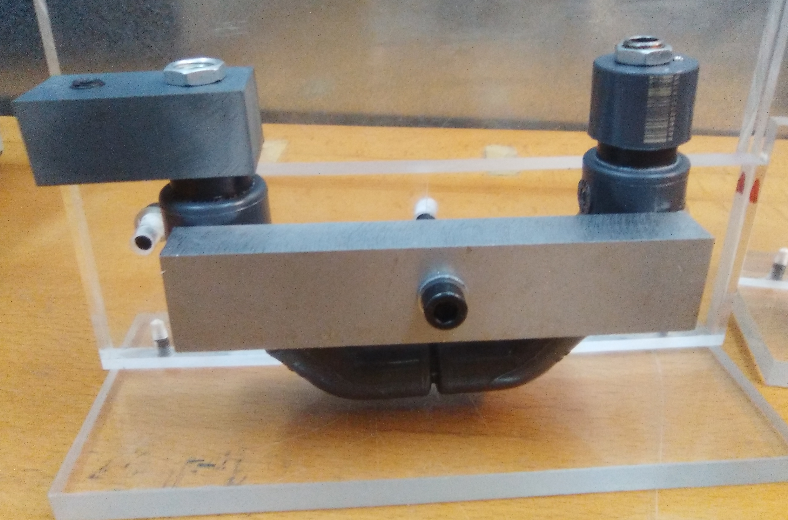
\includegraphics[scale=0.3]{Prototipo.png}
\caption{ Prototipo Tritium\label{prototipo}}
\end{figure}
Este prototipo tiene un volumen interior que permite rellenarlo con   $39~\cm^3$ de solución radiactiva, el cual se calculó y verificó mediante varios ensayos de llenado con agua destilada. También se verificó la estanqueidad del prototipo mediante ensayos de 2 días. 

Se decidió realizar un prototipo con forma de U. Dado que el prototipo no se trasladará en ningún caso y, teniendo en cuenta que se verificó su estanqueidad, personalmente opino que esta es la forma más segura y que mejor se adapta a las exigencias del prototipo. Las dos aperturas superiores se cerraron  y sellaron con tapones, unos utilizados en fontanería de PVC y otros fabricados para este prototipo en los talleres mecánicos del IFIC. Se eligieron tapones diferentes para cada extremo. Un primer tapón circular,  correspondiente al tubo de PVC y un segundo tapón cuadrado, diseñado para facilitar el proceso de llenado. Este segundo tapón dispone de  un orificio de $8~\milli\meter$ por el que se realizó el proceso de llenado  mediante una pipeta. Al primer tapón  se le ha practicado  un orificio de $1~\milli\meter$ para purgar el aire durante el  proceso de llenado. Finalmente, estos orificios se cerraron con  tornillos de rosca envueltos en teflón, y finalmente se sellaron con silicona. Estos tapones se muestran en la figura~\ref{tapones}.
Además, a ambos tapones se les ha practicado un agujero de $9.8~\milli\meter$ de diámetro, tamaño justo para que por cada uno de éstos pase un extremo del haz de fibras centelleadoras. En cada extremo se dispusieron dos arandelas, roscadas al aro que conformaba el extremo del haz de fibras, según se muestra  la figura~\ref{prototipo} (una tuerca interior y otra exterior). De esta forma conseguíamos fijar perfectamente cada uno de los extremos del haz al prototipo y conectar el extremo de las fibras con los fotosensores, PMTs en nuestro caso para la primera etapa de estudi ode estos prototipos. 
También podemos observar que se realiza el giro de $180\degree$, correspondiente a la U, con ayuda de cuatro codos de $45\degree$ y no con dos codos de $90\degree$. Esto es debido a que, con giros progresivos, el haz de fibras centelleadoras está sometidos a una tensión inferior y, por extensión, producirá una mejor propagación de la señal luminosa.

\begin{figure}[hbtp]
\centering
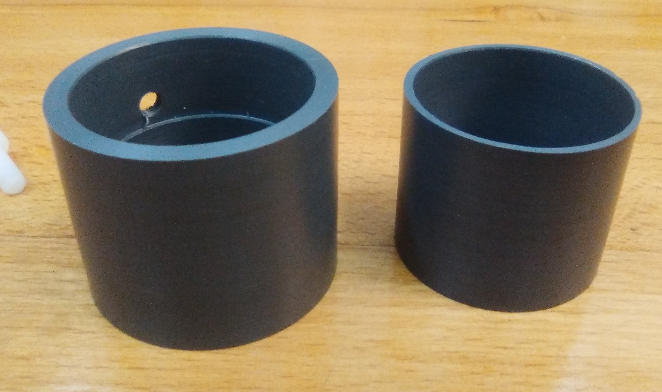
\includegraphics[scale=0.4]{Tapones.png}\\
\caption{ Piezas de sujeción de los PMTs\label{tapones}
}
\end{figure}



Finalmente se utilizaron dos piezas, usualmente utilizadas en fontanería de PVC para comunicar tuberías de igual o diferente diámetro, para sostener los PMTs en el prototipo. Como hemos utilizado dos tapones distintos, necesitamos dos piezas diferentes, mostradas en la figura 21.
La primera pieza (correspondiente a la pieza derecha de esta figura), más pequeña, simplemente encaja en el  tapón circular por un extremo y, por el otro, con un diámetro interior más grande, se dispone el PMT.
Para la segunda pieza encontramos un problema debido a la forma cuadrada del tapón, por lo que utilizamos una pieza  que encaja en la tuerca que sobresale del prototipo (utilizada para fijar el haz de fibras) y por el otro extremo  en  el PMT. Para mejorar la sujeción, se fijó  esta pieza  mediante un tornillo  al soporte de metacrilato. La disposición de los PMT en el prototipo y el tornillo que ayuda a la sujeción pueden verse  en  la figura~\ref{prototipotapones}.

\begin{figure}[htb]
\centering
{
%\subfloat[Espectro de emisión]
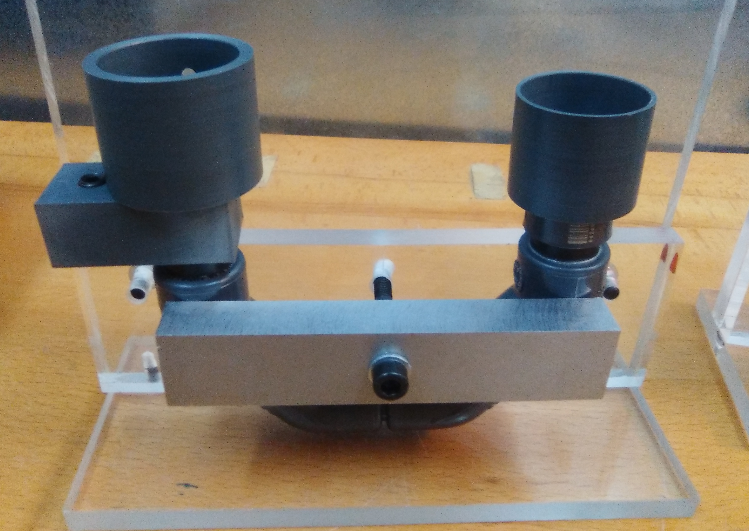
\includegraphics[scale=0.25]{Prototipodelantetapon.png} 
}
{
%\subfloat[Espectro de emisión]
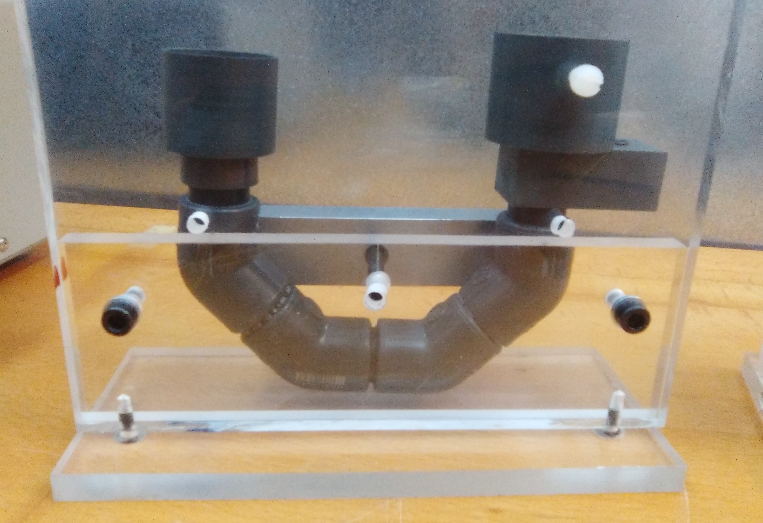
\includegraphics[scale=0.25]{PrototipoDetrastapon.png} 
}
\caption{Prototipo con piezas de sujeción. Vista frontal (izquierda) y vista trasera (derecha) \label{prototipotapones}}
\end{figure} 

Hay que tener en cuenta que el proceso de medida se desarrolla en el interior de una cámara oscura, que  protege los fotosensores  de la  luz exterior. En esta no hay un control de la temperatura como en el sistema utilizado para la calibración de los SiPM. En su lugar únicamente activamos el aire acondicionado en el laboratorio para mantener una temperatura constante de aproximadamente $25~\celsius$ en todo momento.

Los PMTs empleados, Hamamatsu R8520-ZB2771 y R8520-ZB2773, se alimentaron ambos a $-830~\volt$ . A esta temperatura poseen  una ganancias de $G_1=1456178$ y $G_2=1921595$ y sus eficiencia cuantica a $\lambda=430~\nano\meter$ son del $29.76\%$ y $28.66\%$, respectivamente. 
